%!TEX root = ../dissertation.tex

\chapter{Implémentation}
\label{chp:impl}

%Example of \autoref{tab:1}, made using %\url{https://www.tablesgenerator.com/}.


%\begin{table}
%    \centering
%    \begin{tabular}{@{}ll@{}}
%        \toprule
%        \textbf{A} & \textbf{B} \\ \midrule
%        1          & 2          \\
%        3          & 4          \\ \bottomrule
%    \end{tabular}
%    \caption{Interesting results.}
%    \label{tab:1}
%\end{table}

\section{Interface Utilisateur : prototypage}

La conception de notre interface utilisateur étant basée sur la conception centrée sur l'utilisateur, nous présentations dans cette partie la dernière phase de celle ci: L'implémentation.

Nous avons utilisé l'approche Hi-Fi ( High Fidelity) pour le prototypage de nos interfaces utilisateur. Il s'agit d'une représentation avec un maximum de détails.
\subsection{Outils Utilisés pour le prototypage}
\subsubsection{Pour le prototypage}
Notre choix s'est porté sur l'outil \textbf{Figma}. En effet,
\begin{itemize}
    \item Figma est un outil de prototypage en ligne avec une fonctionnalité de collaboration en temps réel.
    \item Il n'est pas nécessaire d'enregistrer et d'organiser les fichiers. Le travail est automatiquement enregistré dans un espace partagé dans le Cloud.
    \item On peut partager tout les prototypes créés en un click.
\end{itemize}

\subsubsection{Pour les illustrations}
La totalité des illustrations présentes sur nos interfaces proviennent du site web \textbf{\href{https://storyset.com/}{Storyset}}.

\subsection{Quelques interfaces réalisées}
\subsubsection{Interface de la création de compte}
Nous présentons à la figure \ref{fig:in_compte}  , l'interface qui sera vue par l'utilisateur lors de la réalisation du cas d'utilisation "Créer un compte".
\begin{figure}[H]
    \centering
    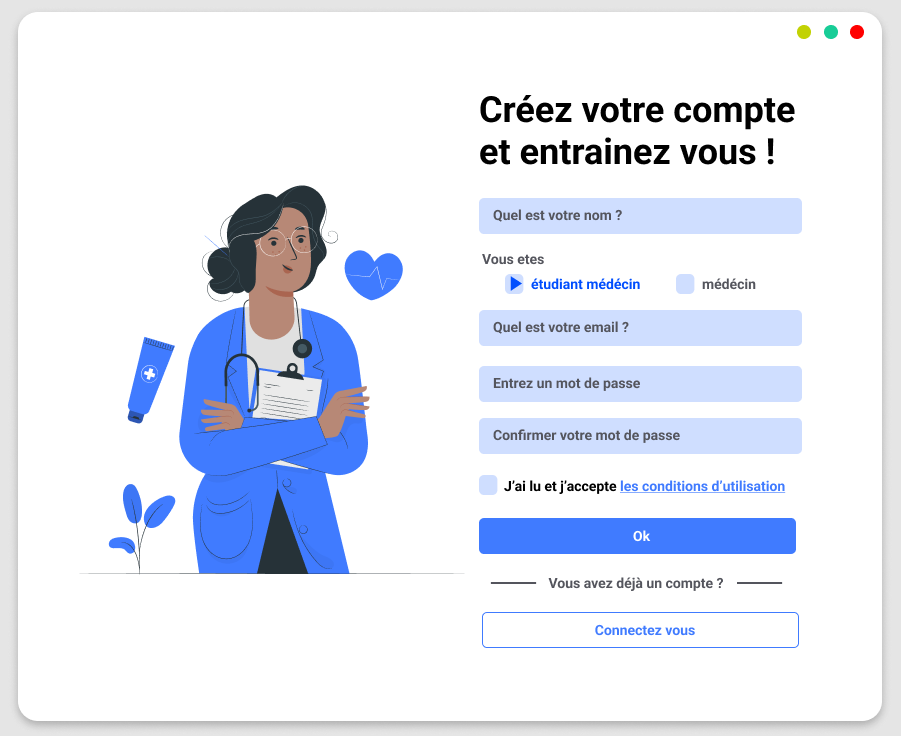
\includegraphics[width=\textwidth]{figures/signup.png}
    \captionsetup{justification=centering}
    \caption{Interface pour la création de compte}
    \label{fig:in_compte}
\end{figure}

\subsubsection{Interface de connexion}
Nous présentons à la figure \ref{fig:in_connection}  , l'interface qui sera vue par l'utilisateur lors de la réalisation du cas d'utilisation "Se Connecter".
\begin{figure}[H]
    \centering
    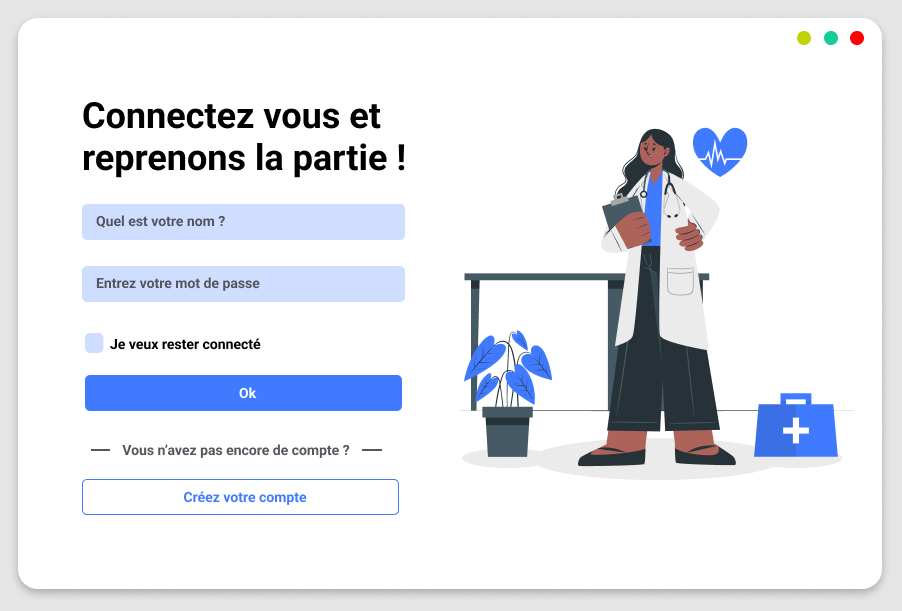
\includegraphics[width=\textwidth]{figures/signin.png}
    \captionsetup{justification=centering}
    \caption{Interface de Connexion}
    \label{fig:in_connection}
\end{figure}

\subsubsection{Interface du tableau de bord à la première connexion de l'utilisateur}
À la première connexion de l'utilisateur, un pré-test lui sera proposé afin de jauger son niveau pour la configuration de son premier exercice de diagnostic. À la figure \ref{fig:dashboard_first}, nous présentons l'interface qui sera vu par l'utilisateur.
\begin{figure}[H]
    \centering
    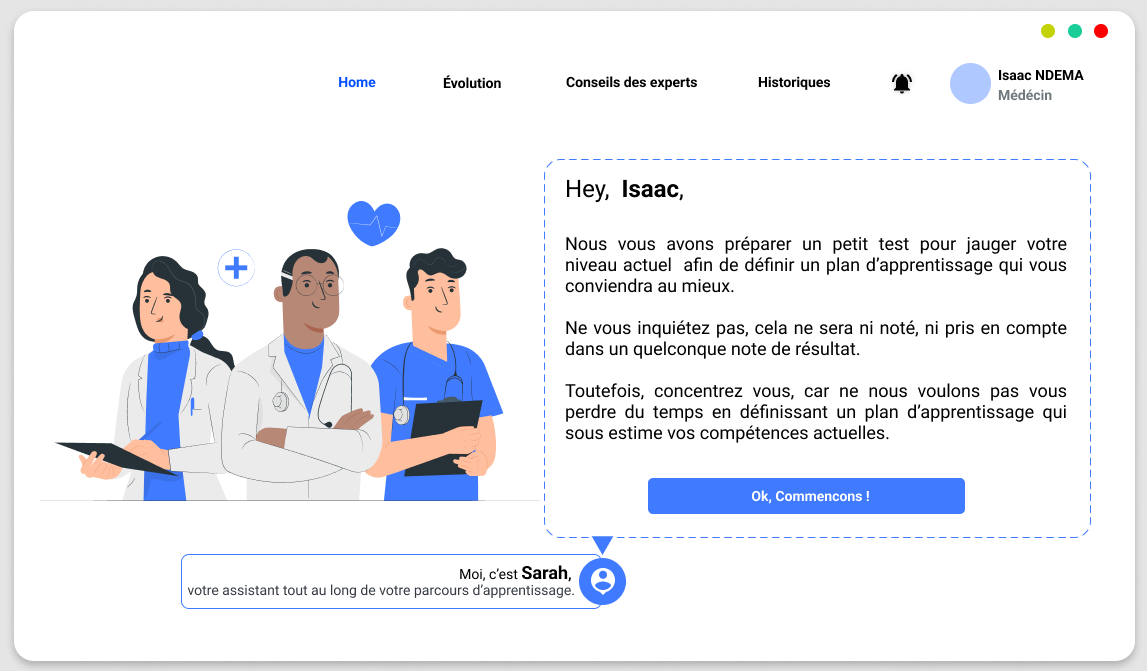
\includegraphics[width=\textwidth]{figures/dashboard-first-connection.png}
        \captionsetup{justification=centering}
    \caption{Inteface du tableau de bord à la 1ère connexion}
    \label{fig:dashboard_first}
\end{figure}

\subsubsection{Interface du tableau de bord  de l'utilisateur}
Nous présentons à la figure \ref{fig:dashboard} , l'interface qui sera vue par l'utilisateur lors de la réalisation du cas d'utilisation "Lancer un exercice de diagnostic".
\begin{figure}[H]
    \centering
    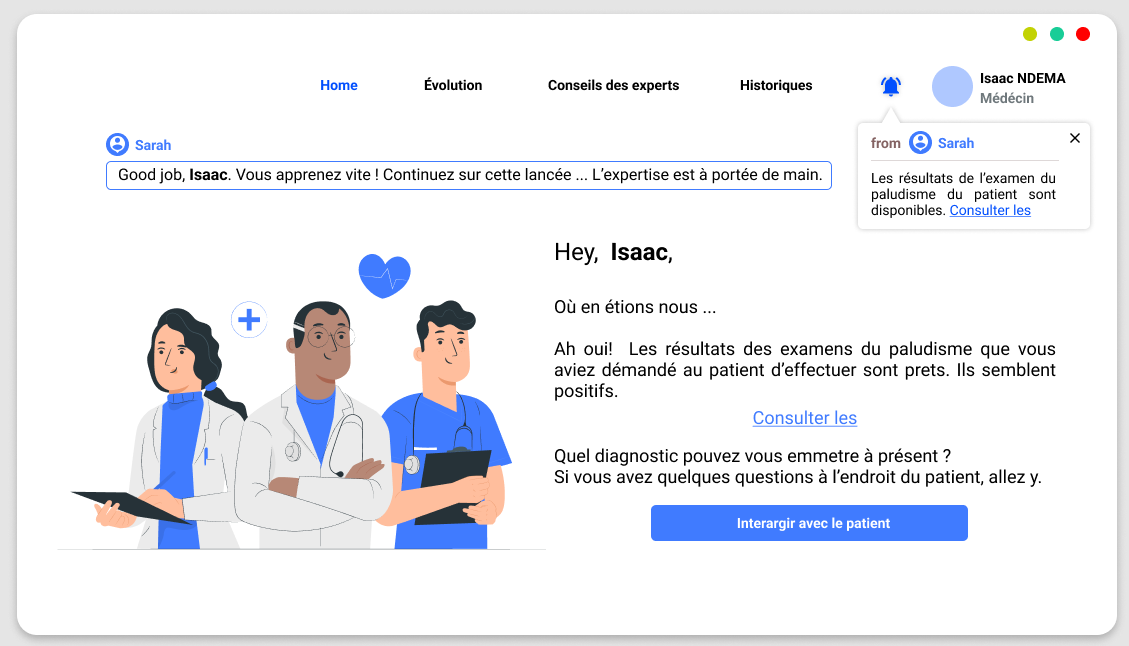
\includegraphics[width=\textwidth]{figures/dashboard.png}
        \captionsetup{justification=centering}
    \caption{Inteface du tableau de bord}
    \label{fig:dashboard}
\end{figure}

\subsubsection{Interface de l'échange entre l'apprenant et le patient virtuel}
Nous présentons à la figure \ref{fig:echange} , l'interface qui sera vue par l'utilisateur lors d'un échange avec le patient virtuel.
\begin{figure}[H]
    \centering
    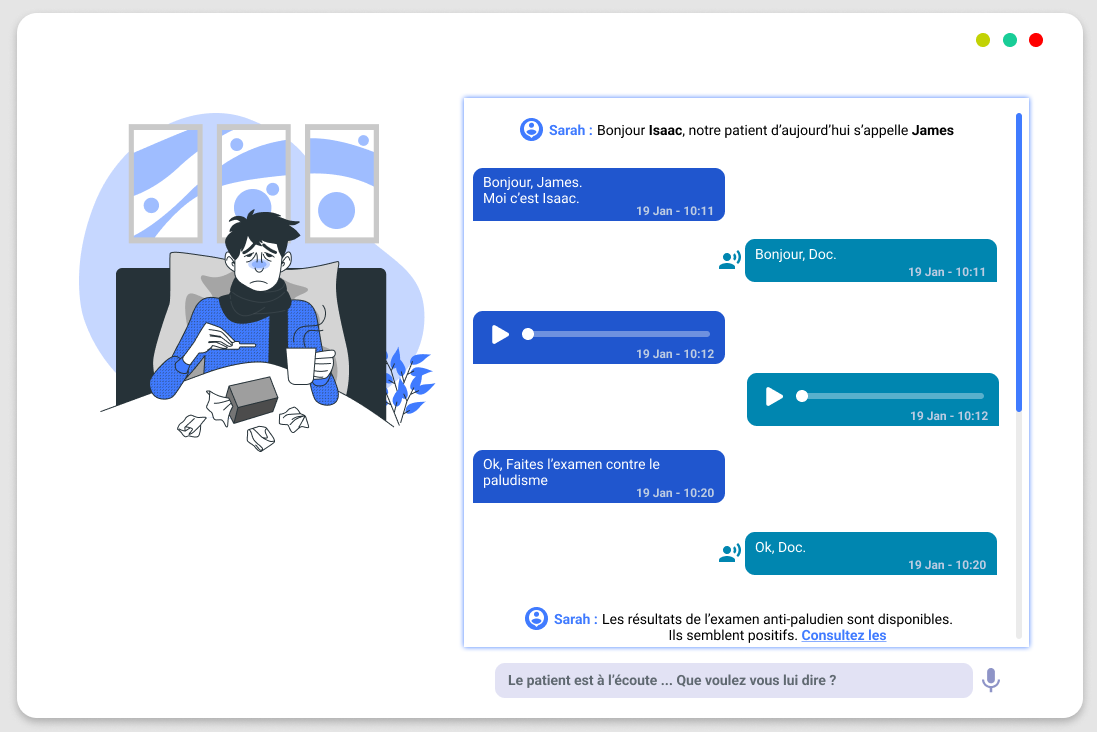
\includegraphics[width=\textwidth]{figures/patient-apprenant.png}
        \captionsetup{justification=centering}
    \caption{Inteface de l'échange entre l'apprenant et le patient virtuel}
    \label{fig:echange}
\end{figure}





\newpage


\section{Tuteur}

Dans les STI, le tuteur joue un rôle très important. Il supervise, oriente et évalue l'apprenant tout au long du processus d'apprentissage. C'est la composante des STI qui implémente l'adaptabilité du système en
offrant la possibilité d'encadrer chaque apprenant de manière personnalisée à travers des interactions soigneusement élaborées.

Dans notre système, les interactions entre le tuteur et l'apprenant se font selon une approche de \textbf{Coaching}, qui est une méthode d'enseignement dans laquelle le tuteur et l'apprenant collaborent à la construction de solutions \cite{vanlehn1996conceptual}. Dans cette méthode l'interaction apprenant-tuteur s'ajuste en fonction des progrès de l'apprenant. 

Pour être capable de remplir efficacement ses fonctions, le comportement de notre tuteur se base sur des règles tutorielles. Par exemple:
\begin{itemize}
    \item Si l'apprenant pose une question pas appropriée, alors l'interpeller et lui rappeler (donner une piste) les types de questions à poser dépendant du contexte.
    \item Si l'examen demandé par l'apprenant ne cadre pas avec le contexte, alors l'interpeller et l'orienter si nécessaire.
    \item Si le différentiel proposé par l'apprenant est trop éparse et divergeant, alors l'interpeller et l'orienter si nécessaire.
\end{itemize}


Pour implémenter ces règles nous proposons l'outil \textbf{JESS} (Java Expert System Shell) qui est une API entièrement développée en Java pour la création des systèmes experts à base de règles.